\chapter{Resultados}

\section{Sistema simulado}

Los sistemas se simularon a las temperaturas de: 280 K, 298.15 K, 310 K, 320 K, 330 K, 340 K, 350 K, 360 K y 370 K; con las siguientes caracteristicas:

\begin{itemize}
    \item Número de moléculas: 16807 moléculas de agua, 10 moléculas de ácido 2,4-diclorofenoxiacético (2,4-D) y un nanotubo de carbono (6, 5) con 364 átomos.
    \item Integrador de todos los sistemas: salto de rana para las ecuaciones de movimiento de Newton.
    \item Paso de tiempo: 0.002 ps, número de pasos: 10000000, Intervalo de tiempo: 20 ns.
    \item radio de corte para la lista de vecinos de corto alcance: 1.2 nm, radio de corte para interacción de coulomb: 1.2 nm, radio de corte para interacción LJ 12-6: 1.2 nm.
    \item Corrección de dispersión de largo alcance para energía y presión.
    \item Acoplamiento de temperatura: ensamble extendido de nose-hoover con $\tau_t$: 0.4 ps y con las temperaturas antes mencionadas.
    \item Acoplamiento de presión: ensamble extendido de parrinello-rahman con $\tau_p$: 1.6 ps a presión: 1 bar.
    \item Algoritmo de constricción: LINCS(LINear Constraint Solver).
\end{itemize}

El campo de fuerzas usado en el sistema es GROMOS 54A7, que tiene generalmente la siguiente forma:

\begin{equation}
\begin{split}
    &{U}_{GROMOS}(r_{ij},\theta_{ijk},\phi_{ijkl})\\ & = \sum_{enlaces}\frac{1}{4}k_{ij}^{b}(r_{ij}^2 - b^{2}_{ij}) + \sum_{angulos} \frac{1}{2}k^{\theta}_{ijk}\Big(cos(\theta_{ijk}) - cos(\theta^{0}_{ijk})\Big)^2\\ 
    &+ \sum_{diedros\ impropios}\frac{1}{2}k^{\xi}_{ijkl}(\xi_{ijkl} - \xi_{0})^2 + \sum_{diedros}k^{\phi}_{ijkl}\Big(1 + cos(n\phi_{ijkl} - \phi^{s}_{ijkl}) \Big)\\ 
    &+ \sum_{pares\ atomos}\left[4\epsilon_{ij} \left[\left(\frac{\sigma_{ij}}{r_{ij}} \right)^{12} - \left(\frac{\sigma_{ij}}{r_{ij}}\right)^6 \right] + \left(\frac{q_i q_j}{4\pi \epsilon_{0} r_{ij}}\right)\right]
    \end{split}
\end{equation}

Con n=2 al menos que se especifique lo contrario en el apéndice 1.

\section{Gráficas}

A continuación se presentan gráficas para analizar el sistema estudiado.

\subsubsection{Propiedades termodinámicas}

Se muestran algunas figuras que son cálculos instantáneos de la presión y temperatura:

\begin{figure}[!h]
    \centering
    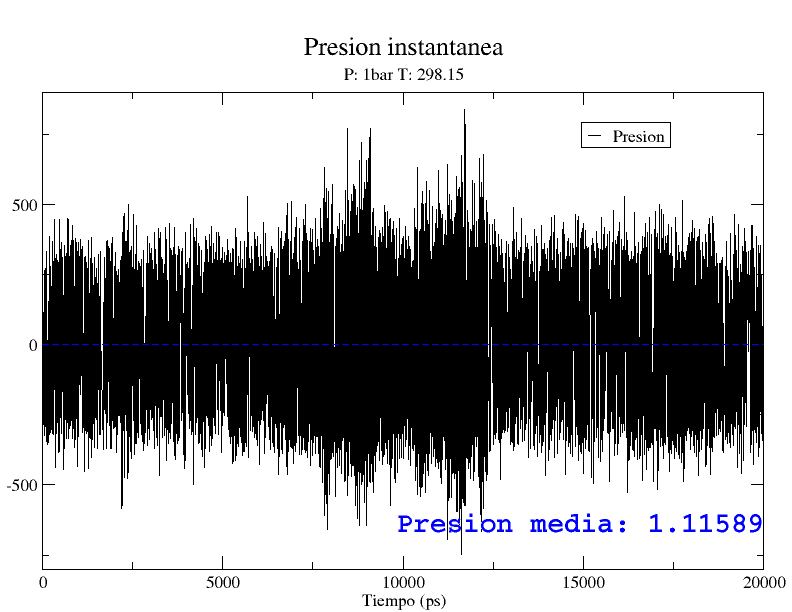
\includegraphics[width=.9\textwidth,keepaspectratio=true]{Pres298.png}
    \caption{Gráfica de la presión instantánea del sistema a condición estandar IUPAC, la media de la presión fue 1.11589 bar}
    \label{fig:Enertot298.15}
\end{figure}

\subsubsection{Función de distribución radial}
